\section{Results}
We study a tri-trophic system over a period of time from spring to fall, in order to capture the seasonal variations in population levels and vertical migrations. We restrict ourselves to a single seasonal cycle so we do not have to take the radically changed resource dynamics during winter into account, and can avoid questions of hibernation and other seasonal adaptations for low-resource environments. We compare three different cases of behavioral optimization: Full rationality, ($\sigma = 0 m^2$), bounded rationality ($\sigma = 10 m^2$), and a fully irrational system with a uniform distribution throughout the water column $(\sigma = \infty m^2)$ as a reference. The system with a uniform distribution reduces our dynamic to Lotka-Volterra dynamics and is included as a reference system, to showcase the dynamics without behavior.

\subsection*{Population dynamics}
\begin{figure}[H]
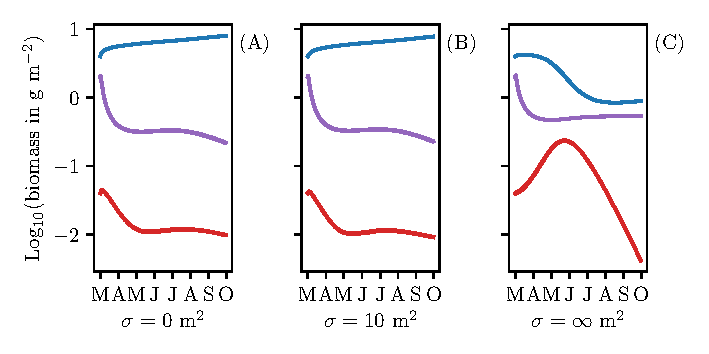
\includegraphics{plots/populations.pdf}
\caption{Total populations of consumers \emph{(blue)}, predators, \emph{(red)} and resources \emph{(purple)} from 1st of april to 1st of october. We vary the rationality, from total rationality \emph{(A)}, bounded rationality ($\sigma = 10$), \emph{(B)} and fully irrational, $\sigma = \infty$, \emph{(C)}, corresponding to a simple Lotka-Volterra model.}
\label{fig:long_term_populations}
\end{figure}
\Cref{fig:long_term_populations} shows the seasonal-term population dynamics for the system we consider, comparing the population levels for the models with complete rationality (\Cref{fig:long_term_populations}(A)), bounded rationality (\Cref{fig:long_term_populations}(B)) and full irrationality (\Cref{fig:long_term_populations}(C)).

In the system with full irrationality \Cref{fig:long_term_populations}(C) we see very unstable population dynamics, with the consumer population crashing and the predator population in the middle of a crash at the end of the simulation. In contrast, both bounded and full rationality result in stable population dynamics (\Cref{fig:long_term_populations}(A,B)). All three models have an initial large population growth, but the behavioral optimization rapidly dampens the population dynamics, as the increase in predator populations leads to a corresponding decrease in the willingness of consumers to take risks (\Cref{fig:long_term_populations}(A,B)). In the summer, the effect of a much shorter night is visible in the resource dynamics on the long term (\Cref{fig:long_term_populations}(A,B, (J, J), purple)), since the resource population increases, leading to more risk-willing consumers and a higher predator-population (\Cref{fig:long_term_populations}(A,B, (J, J), red)). Surprisingly this is not enough to counter the rise in consumer numbers (\Cref{fig:long_term_populations}(A,B, (J, J), blue)).

 The population levels for the model with bounded and full rationality are essentially indistinguishable, so the decrease in fitness from the decrease in optimality is not that great. Viewed on a long time-scale the underlying daily variation is practially invisible.
% The resources reach a stable level quickly in all three cases, but the populations of consumers and predators differ markedly. The difference in populations between the system with bounded rationality \Cref{fig:long_term_populations}(2) and the fully rational system appears to be negligible, \Cref{fig:long_term_populations}(1). The main driver of the change in population dynamics seems to be the ability to retreat to a refuge, and not the exact shape of the distributions when interacting.

\subsection*{Bounded rationality and complete rationality}
\begin{figure}[H]
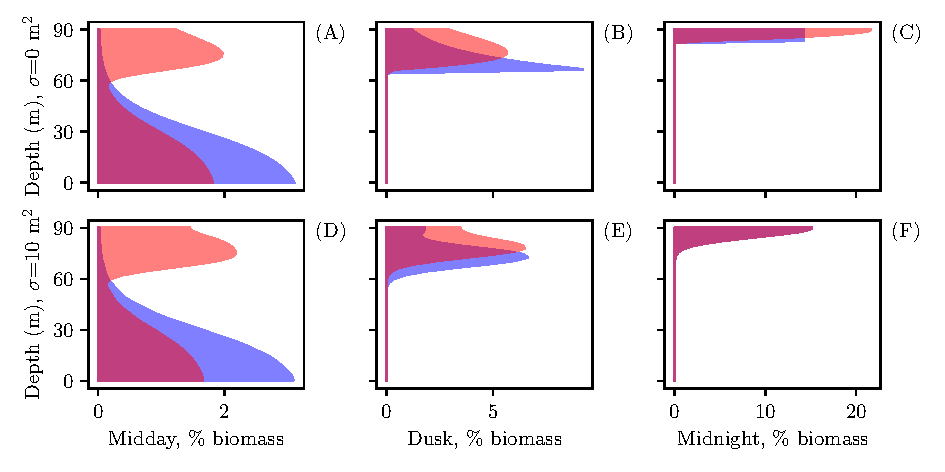
\includegraphics{plots/both_specific_dists.pdf}
\caption{Daily distribution of consumers \emph{blue} and predators \emph{red} at noon \emph{(A,D)}, dusk \emph{(B,E)} and at midnight, \emph{(C,F)} with full (A-C) and bounded rationality (D-F) on the 22nd June (Summer solstice)}
\todo[inline]{... og ressource ...}
\label{fig:both_specific_dists}
\end{figure}
The plots in \Cref{fig:both_specific_dists} show snapshots of consumer and predator distributions in the water column at dawn, midday and dusk on summer solstice. $\Cref{fig:both_specific_dists} (A-C)$ shows the distributions with full rationality, and $\Cref{fig:both_specific_dists} (D-F)$ show the migration with bounded rationality. Any significant differences in behavioral choices between our model of bounded rationality and full rationality become visible when viewing the resulting distributions simultaneously. As expected, a pattern of vertical migration emerges with the emergence of a deep scattering layer of fully rational consumers at noon \Cref{fig:both_specific_dists}(A, blue). Most of the predators are also present in this layer \Cref{fig:both_specific_dists}(A, red), excepting a few hanging out higher in the water column deterring upward consumer migration, corresponding to the modelling results of \citep{jerome}. At dusk, \Cref{fig:both_specific_dists}(B) the predators have a greater concentration near the surface, while the consumer "box" is begining to form, yet still with a continuous drop-off to the surface due to the risk from the light. At midnight \Cref{fig:both_specific_dists}(C) the consumers are concentrated near the surface, with a discontinuous drop to nothing. The predators follow the consumers, albeit with a continuous shape, both distributions being similar to the results of \citep{verticalmigration}.


The behavioral choices with bounded and full rationality are strikingly similar, especially at noon (\Cref{fig:specific_dists_rational}(A, D)). At dusk a the consumers with full rationality have a large discontinuous peak in their distribution, which declines continuously towards the top of the water column due to the risk from light (\Cref{fig:specific_dists_rational}(B, blue)), while the consumers with bounded rationality follow the same overall pattern of moving towards the surface, (\Cref{fig:both_specific_dists}(E, blue)). The increased concentration of consumers with bounded rationality at the top of the water column (\Cref{fig:both_specific_dists}(E, blue)) must be balanced by the wider breadth of the consumer distribution. Due to the slightly higher concentration of bounded rationality consumers at the top, predators with bounded rationality have a peak in their distribution slightly higher in the water column than the fully rational ones (\Cref{fig:specific_dists_rational}(B, E, red)). Apart from the location, the predator distributions are otherwise quite alike, with the rational predators having an emergent almost-smooth distribution.
At midnight the distribution of fully rational consumers has a discontinuous dropoff (\Cref{fig:both_specific_dists}(C, blue)). Due to the forced dispersion, the consumers with bounded rationality are more spread out (\Cref{fig:both_specific_dists}(F,blue)), but the distribution looks like a smoothed version of the fully rational distribution.
In contrast to the consumers, the fully rational predators and the predators with bounded rationality have almost the same distribution, where they spread out at night, with the highest concentration in the top of the water column (\Cref{fig:both_specific_dists}(C, red)).

%As both predators and consumers follow the Nash equilibrium strategy, their fitness is identical at the various points in the water column due to the behavioral choices.


%At noon, \Cref{fig:both_specific_dists}(A) the consumers form a deep scattering layer, where most of the predators are also present. excepting a few hanging out higher in the water column deterring upward consumer migration \Cref{fig:specific_dists_rational}(1)(15 m), corresponding to the modelling results of \citep{jerome}.

%At dusk, \Cref{fig:both_specific_dists}(B) the predators have a greater concentration near the surface, while the consumer "box" is begining to form, yet still with a continuous drop-off to the surface due to the risk from the light. At midnight \Cref{fig:both_specific_dists}(C) the consumers are concentrated near the surface, with a discontinuous drop to nothing. The predators follow the consumers, albeit with a continuous shape, both distributions being similar to the results of \citep{verticalmigration}.

%Examining the migration in the ecosystem with bounded rationality, \Cref{fig:specific_dists_irrational}(D-F), we see roughly the same picture as in \Cref{fig:specific_dists_rational}(A-C). The greatest difference is at midnight and dusk, \Cref{fig:specific_dists_irrational}(B,E,C,F), where the bounded rationality leads to a smooth shape for the distrbution of consumers. At noon, the distributions in the system with bounded rationality \Cref{fig:specific_dists_irrational}(D) and perfect rationality \Cref{fig:specific_dists_rational}(A) are almost entirely equal.

\subsection*{Seasonal variation}
\begin{figure}[H]
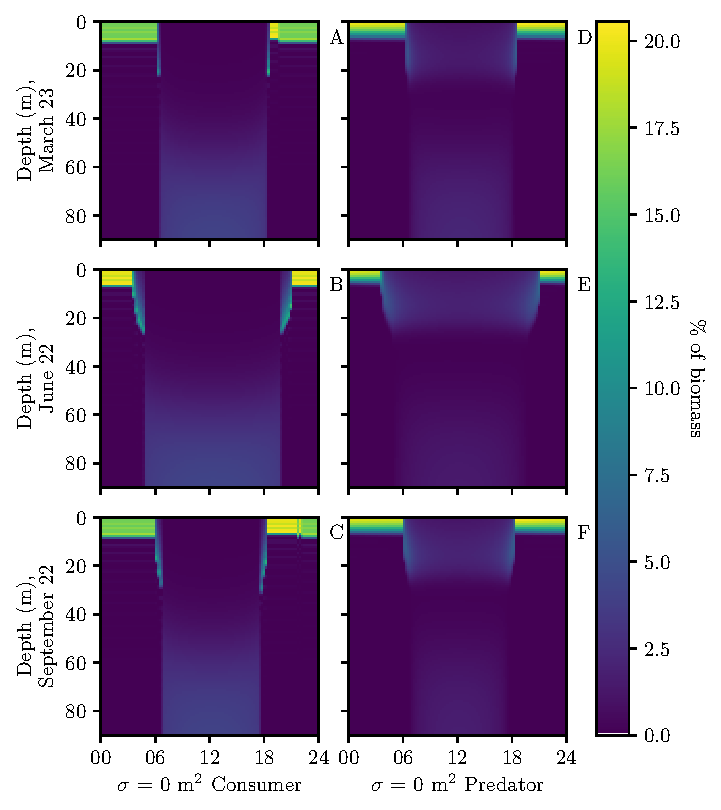
\includegraphics{plots/total_heatmap.pdf}
\caption{Vertical distribution of consumers \emph{(A-C)} and predators \emph{(D-F)} at spring equinox (March 22), summer solstice (June 22) and fall equinox (September 23)}
\label{fig:heatmap_total}
\end{figure}
The heatmaps in \Cref{fig:heatmap_total} illustrate the seasonal variation of the daily migration of consumers (\Cref{fig:heatmap_total}(A-C)) and predators (\Cref{fig:heatmap_total}(D-F)), by focusing on the equinoxes and the summer solstice.
%To understand the migration in greater detail, we look at the complete migration picture.
The vertical migration (\Cref{fig:heatmap_total}) is apparent throughout the seasons. Both consumers and predators are highly concentrated at the top of the water column during nighttime, and at day they scatter to the deep, with a transition during dusk as illustrated in \Cref{fig:both_specific_dists}(B,D). Looking at the consumers (\Cref{fig:heatmap_total}(A-C)), there is a clear seasonal variation in the speed of the migration and the size of the consumer "box" at nighttime. In the spring, (\Cref{fig:heatmap_total}(A)) the consumer migration is very fast, due to a relatively large predator population from the initial boom, so each individual consumer is at very high risk in the spring. In addition, the day-night transition is quite fast during the equinox. Predators follow the consumers (\Cref{fig:heatmap_total}(D)), but with a continuous distribution.
At the summer solstice, (\Cref{fig:heatmap_total}(B,D)) the migration has changed character with a more protracted duration, occasioned by a slower change in light levels than in the spring. In addition the predator population has declined a bit from its spring high, and is slowly rising again \Cref{fig:long_term_populations}, leading to a less risky environment for the consumers. The shape of the distributions of predators and consumers is the same as in the spring, with the only major difference being the shape of the migration.

Moving the hands on the clock forward to the fall equinox, we see a different pattern \Cref{fig:heatmap_total}(C,F) compared to the spring equinox. The vertical migration is slower in the fall than the spring, which can be seen by the width of the intermediate states in \Cref{fig:heatmap_total}(C,F). An individual consumer is in less danger than in the spring, due to the decline in predator populations and rise in consumer populations \Cref{fig:long_term_populations}.



%In the spring \Cref{fig:heatmap_total}(A) the consumer migration is very fast, reflecting relatively fast shift in light levels, with a much slower migration in the summer \Cref{fig:heatmap_total}(B,E).
%The pattern of the predators \Cref{heatmap_total}(D-F) is slightly different from the consumer pattern, \Cref{fig:heatmap_total} (A-C). At nighttime there is still a non-zero concentration of predators in the upper layers of the water-column, there to catch any errant prey.
%\todo[inline]{Forskellen mellem forår og efterår bør kommenteres}

\subsection*{Feeding rates}
\begin{figure}[H]
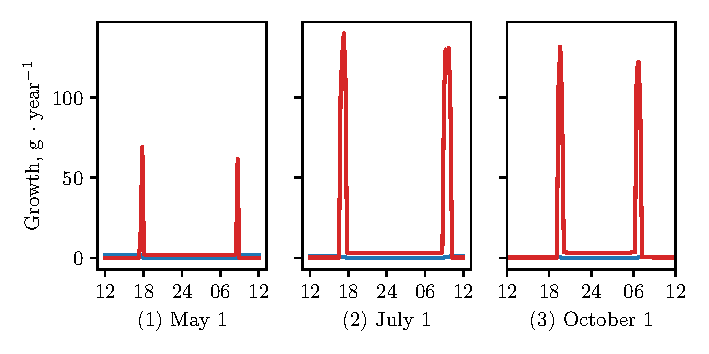
\includegraphics{plots/growth_short_rational.pdf}
\caption{Seasonal comparison of consumer \emph{(blue)} and predator, \emph{(red)} feeding patterns on March 22 (spring equinox) \emph{(A)}, 22 June (summer solstice) \emph{(B)} and 23 of September (fall equinox) \emph{(C)}}
\label{fig:growth_short_rational}
\end{figure}
\Cref{fig:growth_short_rational} shows the seasonal variations in the daily feeding patterns of consumers (blue) and predators (red), by zooming in on the spring equinox, summer solstice and fall equinox.

At all three points in time, consumers have a constant feeding level throughout the night \Cref{fig:growth_short_rational}, due to the vertical migration \Cref{fig:heatmap_total}. In spite of the predator and consumer populations being overlaid at night (\Cref{fig:heatmap_total}(A,C)), the predators have practically no feeding activity at night \Cref{fig:growth_short_rational}. This illustrates the advantage of the diel vertical migration for the consumers.

The main feeding time for predators is at dawn and dusk, \Cref{fig:growth_short_rational}, again illustrating the efficacy of the diel vertical migration as a predator-avoidance strategy for the consumers. In the spring, there is a large amount of predators and not that many consumers, so the individual consumers get to eat more as evidenced by the high peaks \Cref{fig:growth_short_rational}(A,blue), while the individual predators go hungry \Cref{fig:growth_short_rational}(A,red). The duration of predator feeding is largest in the summer (\Cref{fig:growth_short_rational}(B, red)), where we also see the slowest migration (\Cref{fig:heatmap_total}(B,D)). That individual predator feeding is slightly larger in the summer than in the fall is surprising, since there are more predators in the summer (\Cref{fig:long_term_populations}(J,J vs S,O, red)). Consumers increased risk avoidance must also be occasioned indirectly by the increased consumer population from summer to fall leading to less available food, both pr. capita and in total (\Cref{fig:long_term_populations}(A, purple)), and by the longer day-night transition. As the consumer population increases through the seasons, each consumer gets less food during the night \Cref{fig:growth_short_rational}(A-C, blue) due to intraspecific competition, while the predator feeding level stabilizes \Cref{fig:growth_short_rational}(B, D, blue) after the famine (\Cref{fig:growth_short_rational}(A, red)).

\begin{comment}
\begin{figure}[H]
  \begin{centering}
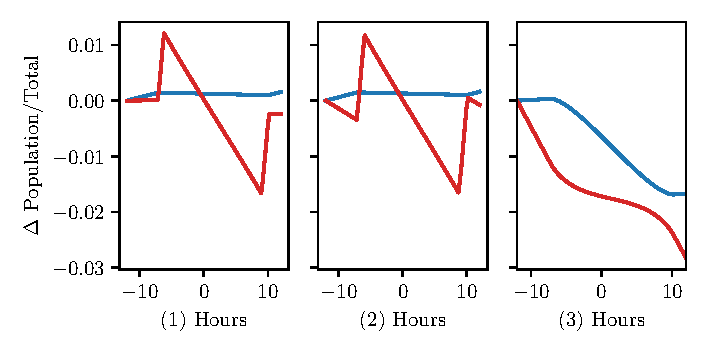
\includegraphics{plots/pop_dyn_comp_full_semi_none.pdf}
\end{centering}
\caption{Comparison of consumer \emph{(blue)} and predator, \emph{(red)} pr. capita growth patterns with complete rationality \emph{(A)}, bounded rationality \emph{(B)} and full irrationality \emph{(C)}}
\todo[inline]{Jeg er ikke helt overbevist af denne figur ... lad os tale om det.}
\label{fig:pop_short_term}
\end{figure}
The differentshort-term population growth patterns for complete rationality, bounded rationality and full irrationality are illustrated in \Cref{fig:pop_short_term}, by focusing on the patterns on summer solstice.
Looking at short-term population growth in the model with complete rationality and bounded rationality, \Cref{fig:pop_short_term}(A,B), the change in consumer and predator populations throughout a day is on the order of $10^{-3}$. In contrast, the model with constant behavior has rather large fluctuations of populations through a single day \Cref{fig:pop_short_term}(C).
\end{comment}

%Compare to behavior visser2001observations, hay1991zooplankton

%Compare to wang2014seasonal, klevjer2016large, olivar2017mesopelagic, beaugrand2001geographical, colebrook1979continuous

%%% Local Variables:
%%% mode: latex
%%% TeX-master: "main"
%%% End:
